% \newcommand{\bh}{\mathbf{h}} 
%\newcommand{\bt}{\mathbf{t}} 
%\newcommand{\bu}{\mathbf{u}} 
%\newcommand{\bv}{\mathbf{v}} 
%\newcommand{\bw}{\mathbf{w}} 
%\newcommand{\bx}{\mathbf{x}} 
%\newcommand{\bz}{\mathbf{z}} 
%\newcommand{\by}{\mathbf{y}} 

\newcommand{\ini}{\text{init}}
\newcommand{\targ}{\text{targ}}
\newcommand{\otdd}{\text{OTDD}}
% \newcommand{\dd}{\text{d}}

\newcommand{\bbW}{\mathbb{W}}

\newcommand{\cZ}{\mathcal{Z}}

\definecolor{molive}{RGB}{169, 158, 38}
\newcommand{\olive}[1]{{\color{molive} #1}}

\definecolor{mpink}{RGB}{218, 123, 225}
\newcommand{\pink}[1]{{\color{mpink} #1}}

\definecolor{myfiol}{RGB}{189, 21, 211}
\newcommand{\fiol}[1]{{\color{myfiol} #1}}

\newcommand{\fdv}[2]{\frac{\delta #1}{\delta #2}}
\newcommand{\divg}[1]{\mathbf{\nabla} \cdot #1}

\newcommand{\dd}{\text{d}}

\newtheorem{Obj}{Objective}

\section{Introduction}

В машинном обучении ключевое положение занимают вопросы о данных, необходимых для запуска любого пайплайна машинного обучения: 
\begin{enumerate}
    \item наличие/отсутствие данных
    \item аугментация данных
    \item введение полезных геометрических свойств в данные (например, linear separability, class separation)
    \item возможность переиспользования моделей, обученных на одних данных, для сторонних данных (например, transfer learning)
    \item domain adaptation
\end{enumerate}
В настоящей работе предлагается фреймворк для решения различных (в т.ч. вышеперечисленных) задач в контексте \textbf{labeled dataset transformation} с помощью градиентных потоков в пространстве вероятностных распределений

\section{References Review}
\begin{itemize}
    \item \cite{pmlr-v139-alvarez-melis21a} - Основная работа, на которой основан настоящий доклад. Приводятся вся основная теория, имеющая отношение к Dataset Dynamics с помощью градиентных потоков, а также рассматриваются несколько приложений Dataset Dynamics к модельным и реальным задачам.
    \item \cite{Santambrogio2015OptimalTF} - Теоретическая работа, посвященная теории оптимального транспорта для градиентных потоков.
\end{itemize}

\section{Main Part}

\subsubsection{Постановка задачи}

Пусть нам дан датасет $D_{\ini} = \{ (x_i, y_i) \}_{i = 1}^{N}$; $x_i \in \cX$ - вектора признаков,  $y_i \in \cY$ - метки классификации. Введём $\cZ = \cX \times \cY$. Мы предполагаем, что $D_{\ini} \sim \rho_{D_{\ini}}(\cZ) \in \cP(\cZ)$

Имея функционал $F : \cP(\cZ) \rightarrow \bbR$, задача \textbf{labeled dataset transformation} формализуется следующим образом: 
\begin{gather*}
    \rho_{D^*} = \min\limits_{\rho \in \cP(\cZ)} F(\rho)
\end{gather*}

Здесь $F(\rho) = \olive{\cV(\rho)} + \sunset{\cW(\rho)} + \twilight{\cT_{\targ}(\rho)}$, где:

\begin{itemize}
    \item $\olive{\cV(\rho)}$ - потенциальная энергия (potential energy). $\olive{\cV(\rho)} = \int_{\cZ}V(z) \dd \rho(z)$. Может быть использована для введения поэлементных ограничений в целевом датасете. 
    \begin{itemize}
        \item $V(z) = \Vert x \Vert$ ограничивает норму вектора признаков $x$ ($z = (x, y)$)
        \item $V(z) = \max\left\{ y(x^{T} w - b) \right\}$ для фиксированных $w$, $b$ вводит линейную отделимость классов (бин. классификация)
    \end{itemize}
    \item $\sunset{\cW(\rho)}$ - энергия взаимодействия (interaction energy). $\sunset{\cW(\rho)} = \int_{Z \times Z} W(z - z') \dd \rho(z) \dd \rho(z')$ вводит нужные взаимодействия между элементами датасета. Например, 
    \vspace{-2mm}
    \begin{gather*}
        W(z) = \begin{cases}\exp \{ - \Vert x - x' \Vert \} & \text{if } y \neq y', \\
        0 & \text{otherwise}\end{cases}
    \end{gather*}
    вводит разделимость классов (многогоклассовый случай)
    \item $\twilight{\cT_{\targ}(\rho)}$ - расстояние до датасета $D_{\targ}$. Подробное определение этого функционала будет приведено в следующей части работы.
\end{itemize}

\subsection{Optimal Transport Dataset Distance}

Введём следующее определение: 

\textbf{Определение}.

 Пусть имеются датасеты $D, D'$, их распределения $\rho_D(\cZ), \rho_{D'}(\cZ')$ соответственно. Пусть $\alpha_D^y(\cX) = \rho_D( \cX | \cY = y)$ - распределение на векторе признаков при фиксированной метке класса $y$ (аналогично для $D'$). Пусть $z \in D$, $z' \in D'$. Определим $d_{\cZ}(z, z') = \left( \Vert x - x' \Vert^2 + \bbW_2^2(\alpha_D^y, \alpha_D^{y'}) \right)^{1/2}$. Тогда расстояние между датасетами $D$ и $D'$ (\textbf{OTDD distance}): 
\begin{gather*}
    \otdd\left(D, D'\right) = \min\limits_{\pi \in \prod\left(\rho_D, \rho_{D'}\right)} \int_{\cZ \times \cZ'} d_{\cZ}(z, z') \dd \pi(z, z')
\end{gather*}

Напомним, что: 

\begin{itemize}
    \item Для $\mu, \nu \in \cP(\cX)$ Вассерштайн-2 расстояние: $\bbW_2^2 = \min\limits_{\pi \in \prod(\mu, \nu)} \int_{\cX \times \cX} \Vert x - x' \Vert^2 \dd \pi(z, z')$
    \item $\pi \in \prod(\mu, \nu) \subset \cP(\cX \times \cX) \Leftrightarrow \forall B \in \cB(\cX): \mu(B) =  \int_{B \times \cX} \dd \pi(z, z') \, ; \, \nu(B) = \int_{\cX \times B} \dd \pi(z, z')$
\end{itemize}

Определим $\twilight{\cT_{\targ}(\rho)} = \otdd(\rho, \rho_{D_{\targ}})$, данный функционал позволяет максимизировать схожесть целевого и искомого датасета в случае задачи классификации. Следует заметить, что использование метрики Вассерштайана $\bbW_2$ между условными per-class распределениями на признаках в качестве расстояния между классами позволяет $\otdd$ метрике быть независимой от того, каким именно образом определены классы в датасете, а основываться исключительно на геометрии порождаемых классами распределений.

Перейдём теперь к методу градиентных потоков Вассерштайна, который позволяет решать поставленную задачу минимизации функционала в пространстве вероятностных распределений.

\subsection{Wasserstein Gradient Flows}

Для начала, введём понятие первой вариации:

\textbf{Определение}

Пусть дан функционал $F : \cP(\cZ) \rightarrow \bbR$. Обозначим $\cM(\cZ)$ как множество мер на $\cZ$ со знаком. Рассмотрим возмущения $\chi \in \cM(\cZ)$ такие, что $\exists \, \varepsilon_0 : \forall \fiol{\varepsilon} \in [0, \varepsilon_0]: \fiol{\rho + \varepsilon \chi} \in \cP(\cZ)$. Если существует такая $\red{G}: \cZ \rightarrow \bbR$, что 
\vspace{-3mm}
\begin{gather*}
    \frac{\dd}{\dd \varepsilon}\cF(\fiol{\rho + \varepsilon \chi})|_{\varepsilon = 0} = \int_{\cZ} \red{G(z)} d \chi
\end{gather*}
для любого такого возмущения $\chi$, то $\red{G}$ называется \textbf{первой вариацией} $F$ в точке $\rho$ и обозначается $\green{\fdv{F}{\rho}(\rho_t)}(\rho)$

\begin{figure}[h]
    \centering
    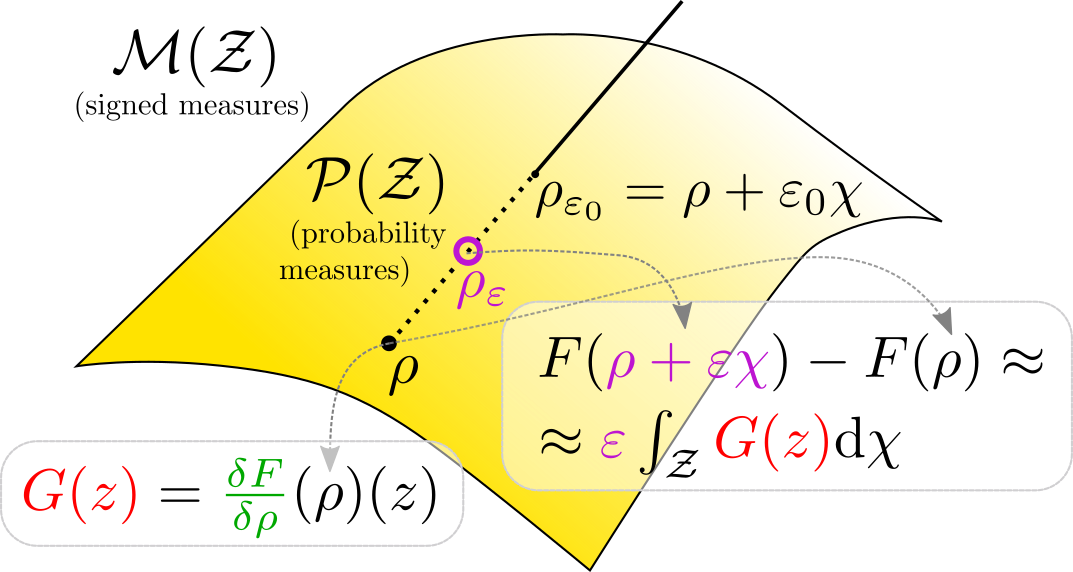
\includegraphics[width=0.5\linewidth]{chapters/petr_mokrov_s2/figs/fv_explanation.png}
\end{figure}

Теперь мы готовы дать определение градиентного потока Вассерштайна. 

\textbf{Определение}

\textbf{Градиентным потоком Вассерштайна} $\{ \rho_t \}_{t \in \bbR_+}$ называется непрерывная последовательность вероятностных мер $\rho_t \in \cP(\cZ)$, удовлетворяющая уравнению непрерывности: 
\begin{gather*}
\begin{cases}
    \partial_t \rho_t \green{- \divg{(\rho_t \nabla_{z} \fdv{F}{\rho}(\rho_t))}} = 0 \\
    \rho_{t = 0} = \rho_{D_{\ini}}
\end{cases}  
\end{gather*}

Верны следующие свойства градиентных потоков: 

\begin{itemize}
    \item $\green{ - \divg{(\rho_t \nabla_{z} \fdv{F}{\rho}(\rho_t)(\rho_t))}} = \nabla_{\bbW_2} F(\rho_t)$, т.е. градиентный поток Вассерштайна - есть "градиентный спуск" в пространстве вероятностных мер.
    \item При некоторых условиях на $F$ градиентный поток Вассерштайна сходится к $\min\limits_{\rho \in \cP(\cZ)} F(\rho)$
\end{itemize}

Последнее свойство позволяет использовать данный метод для решения задачи минимизации целевого функционала.

\subsection{Practical Implementation}

Перейдём теперь к практической реализации построения градиентного потока для Dataset Dynamics. Прежде всего, вычислить нам нужно функционалов первые вариации, что целевой функционал $F$ составляют. 
\subsubsection{First Variation Calculus}

\begin{itemize}
    \item $\olive{\cV(\rho)} = \int_{\cZ}V(z) \dd \rho(z)$ $\Rightarrow$ $\fdv{\olive{\cV}}{\rho}(\rho)(\rho) = V$; 
    % $\hat{V} = \frac{1}{N} \sum\limits_{i = 1}^{N} V(z_i)$
    \item $\sunset{\cW(\rho)} = \int\limits_{Z \times Z} W(z - z') \dd^2 \rho$ $\Rightarrow$ $\fdv{\sunset{\cW}}{\rho}(\rho)(\rho) = 2 \underbrace{\int_{Z}W(z-z') \dd \rho(z')}_{W * \rho}$
    \item  $\twilight{\cT_{\targ}(\rho)} = \otdd(\rho, \rho_{D_{\targ}})$ $\Rightarrow$ $\fdv{\twilight{\cT_{\targ}}}{\rho}(\rho)(\rho) = \varphi_{\rho}$. Здесь $\varphi_{\rho}$ - решение двойственной $\otdd$ задачи Канторовича:
    \vspace{-2mm}
    \begin{gather*} \otdd(\rho, \rho_{D_{\targ}}) = \sup\limits_{\varphi(z) + \psi(z') \leq d_{\cZ}(z, z')} \int\limits_{\cZ} \varphi(z) \dd \rho + \int\limits_{\cZ'} \psi(z') \dd \rho_{D_{\targ}}
    % \makecell{First \\ variation}
    \end{gather*}
\end{itemize}
Таким образом, мы получаем следующий градиентный поток Вассерштайна, с посчитанными вариациями: 
\begin{gather*}
    (\#)\begin{cases}
        \partial_t \rho_t =  \divg{(\rho_t \nabla_{z} (V + W * \rho_t + \varphi_{\rho_t}})) \\
        \rho_{t = 0} = \rho_{D_{\ini}}
    \end{cases}  
\end{gather*}

Градиентному потоку $(\#)$ соответствует следующее стохастическое дифференциальное уравнение:

\begin{gather*}
    \begin{cases}
        \dd Z_t = - \phi(\rho_t, Z_t) \dd t \quad , \,\, \phi(\rho_t, Z_t) = \nabla_{z} (V + W * \rho_t + \varphi_{\rho_t})(Z_t)\\
        Z_0 \sim \rho_{D_{\ini}}
    \end{cases}
\end{gather*}

Имея датасет $\{z_{0}^{(i)}\}_{i = 1}^{N} \sim \rho_{D_{\ini}}$ мы рассматриваем симуляцию элементов этого датасета $z_{k}^{(i)}, k \in \{ 1, 2, \dots T \}$ с помощью \textbf{Forward Euler Scheme} оценивая $\rho_{\gamma k}$ эмпирическим распределением $\sum_{i = 1}^{N}\frac{1}{N}\delta_{z_{k}^{(i)}}$ : 
\begin{gather*}
    z_{k + 1}^{(i)} = z_{k}^{(i)} - \gamma \nabla (V + \widehat{W * \hat{\rho}_{\gamma k}} + \red{\varphi_{\hat{\rho}_{\gamma k}}} ) (z_{k}^{(i)})
\end{gather*}

При этом, для оценки градиентов $\widehat{W * \hat{\rho}_{\gamma k}}$ и $\red{\varphi_{\hat{\rho}_{\gamma k}}}$ мы используем следующее: 
\begin{itemize}
    \item $\nabla \widehat{W * \hat{\rho}_{\gamma k}}(z_{k}^{(i)}) = \sum_{i \neq j} \nabla W(z_{k}^{(i)} - z_{k}^{(j)})$
    \item $\nabla \red{\varphi_{\hat{\rho}_{\gamma k}}}(z_{t}^{(i)}) \rightarrow \nabla_{z_k} \otdd(\hat{\rho}_{\gamma k}, \hat{\rho}_{\targ})$ (интуитивно, $-\nabla \otdd$ направляет элементы изменяющегося датасета в сторону уменьшения $\otdd$, хотя теоретических оснований заменять $\nabla \red{\varphi_{\hat{\rho}_{\gamma k}}}(z_{t}^{(i)})$ на $\nabla_{z_k} \otdd(\hat{\rho}_{\gamma k}, \hat{\rho}_{\targ})$ нам неизвестно)
\end{itemize}

\subsubsection{OTDD gradient estimation}

Для оценки градиента $ \nabla_{z_k} \otdd(D_{\gamma k}, D_{\targ})$ мы используем гауссовскую аппроксимацию $\alpha_D^y \approx \cN(\mu_y, \Sigma_y)$ и $\alpha_D^{y'} \approx \cN(\mu_{y'}, \Sigma_{y'})$. В этом случае $\bbW_2^2(\alpha_D^y, \alpha_D^{y'})$ вычисляется в closed form (как функция от элементов датасета). Далее, 
\begin{itemize}
    \item Оценка $\otdd$ затем вычисляется с помощью OT солверов как функция от элементов датасетов.
    \item При моделировании потока обновляем как элементы датасеты, так и $\mu_y$ и $\Sigma_y$ для различных классов
\end{itemize}

\subsection{Test Cases and Applications}

\subsubsection{Dataset Shaping Test case}

На рисунке ниже представлены эксперименты  с различными целевыми функционалами на синтетическом 3D датасете. В качестве $\olive{\cV}$ используется функционал, вводящий линейную разделимость классов.

\begin{figure}[h]
    \centering
    \hspace*{-5mm}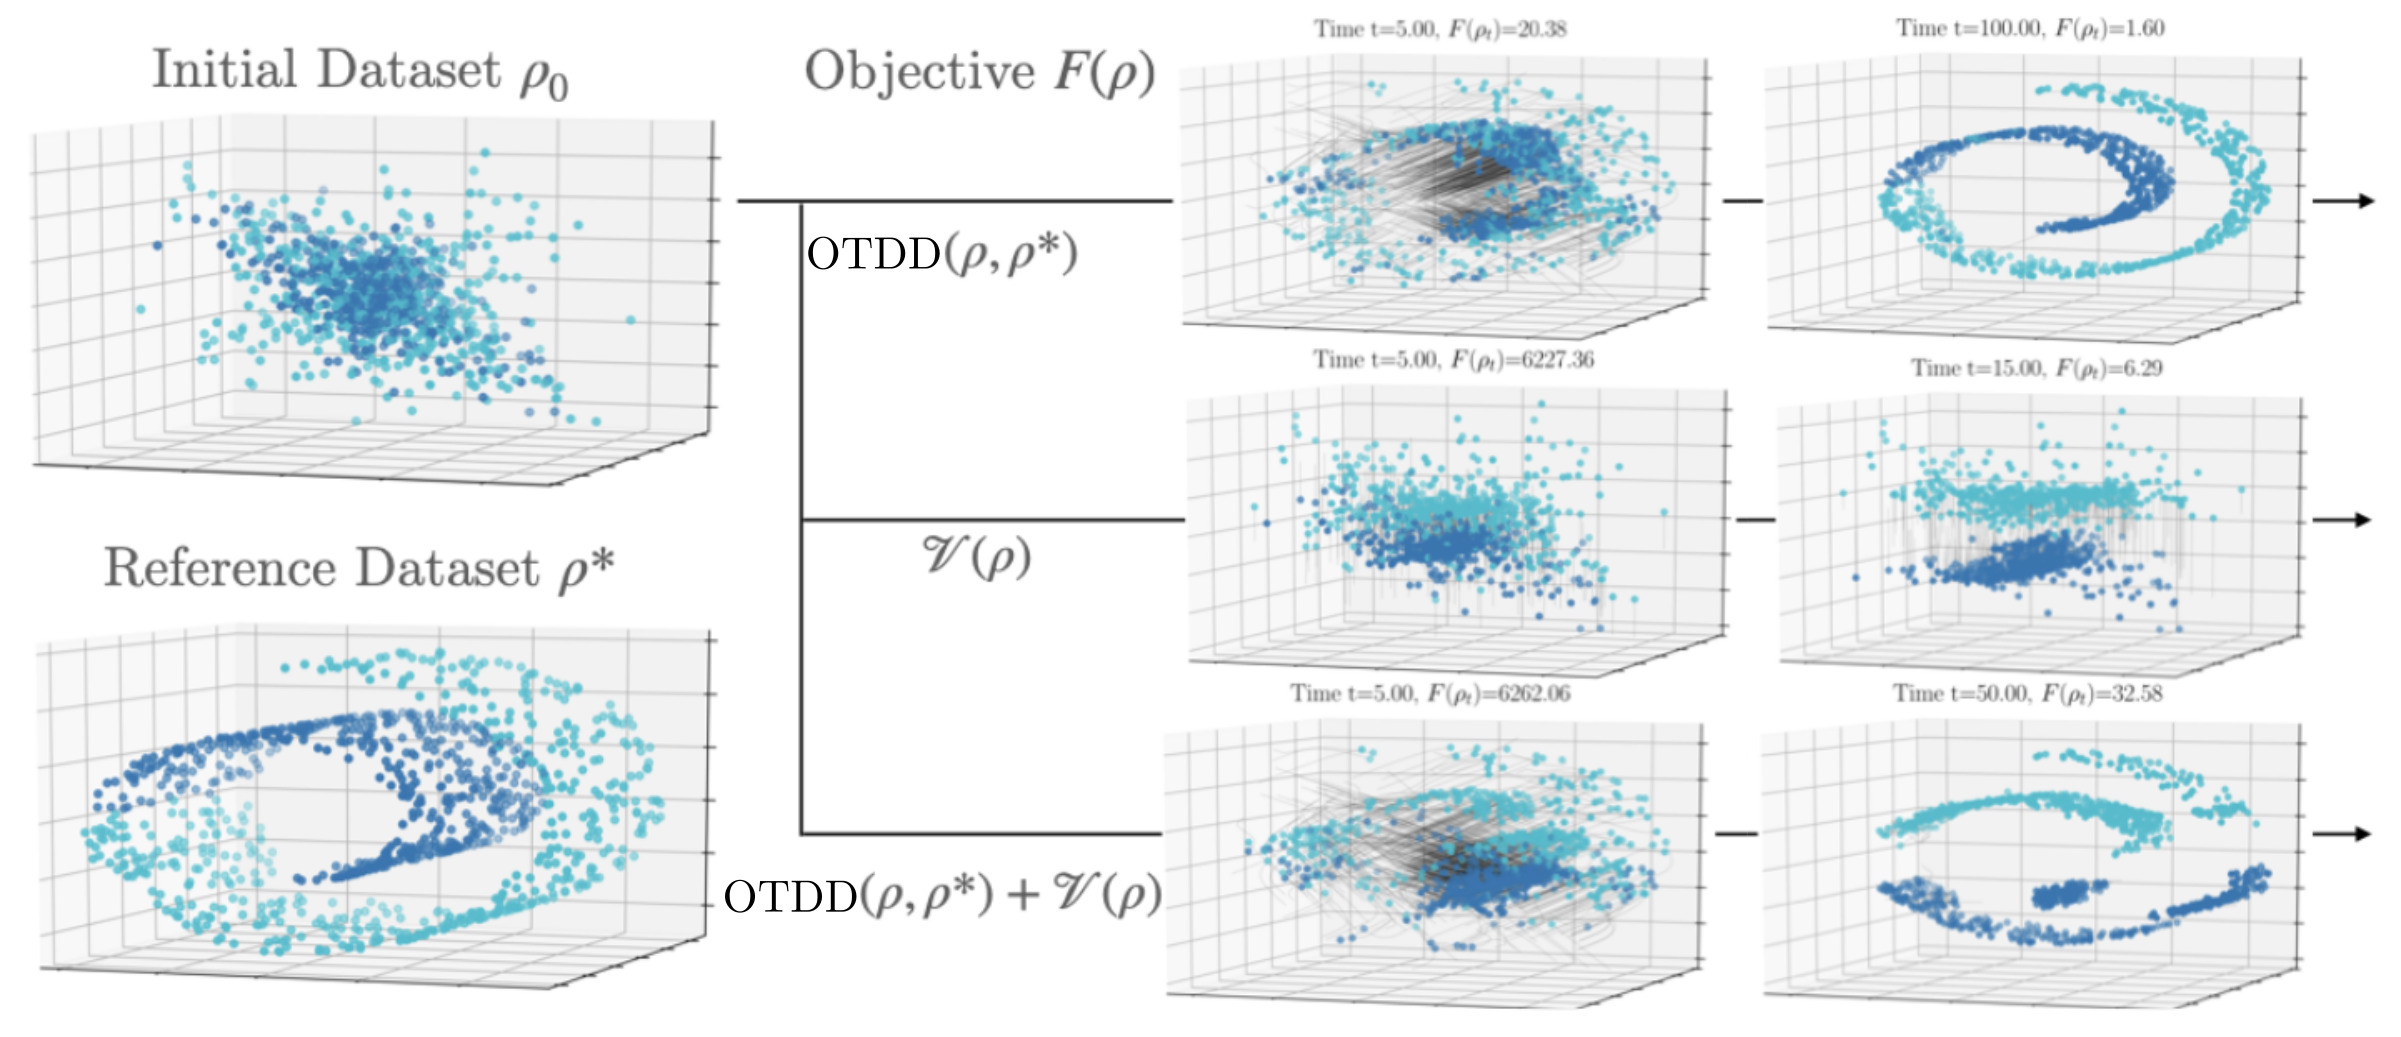
\includegraphics[width=0.9\linewidth]{chapters/petr_mokrov_s2/figs/dataset_shaping_final.png}
\end{figure}

\subsubsection{Transfer Learning Application}

В данном применении мы запускаем градиентные потоки для Transfer Learning попарно между несколькими популярными датасетами для классификации.

В качестве датасетов используются \textbf{M}-MNIST, \textbf{F}-FashionMNIST, \textbf{U}-USPS, \textbf{K}-KMNIST, в качестве функционала служит $F(\rho) = \twilight{\cT_{\targ}(\rho)}$. На рисунке ниже приведена визуализация работы соответствующих градиентных потоков.

\begin{figure}[h]
    \centering
    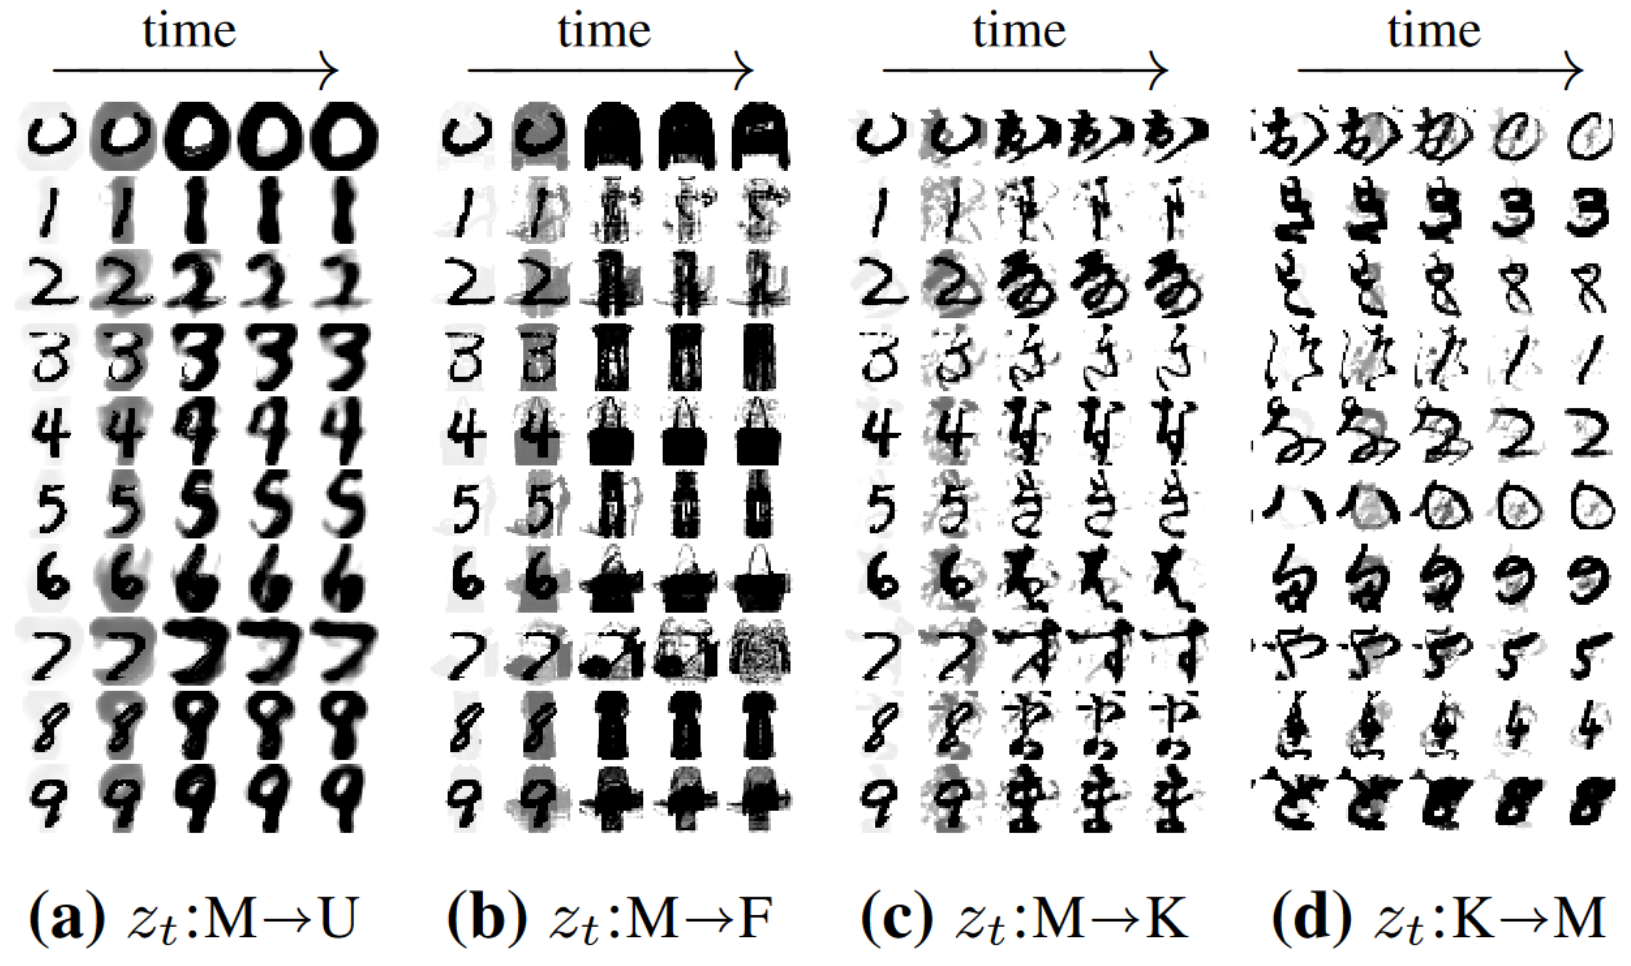
\includegraphics[width=0.7\linewidth]{chapters/petr_mokrov_s2/figs/dataset_dynamics_MKUF.png}
\end{figure}

\subsubsection{Model Repurposing Application}

В данном приложении используется фиксированный классификатор, обученный на $\text{CIFAR10}$ (10 классов), запускается поток $\text{CAMELION (2 класса)} \rightarrow \text{CIFAR10}$ с $F(\rho) = \twilight{\cT_{\targ}(\rho)}$

Для преодоления несоответствия количества классов к классификатору в конце добавляется матрица корресподенций $2 \times 10$ на основе OT между гистограммами вероятностей.

На рисунке ниже представлен результат классификации $\text{CAMELION}$ датасета, преобразованного с помощью градиентного потока, с использованием модели, обученной на $\text{CIFAR10}$. Мы видим, что полученная точность превосходит даже точность базовой модели, обученной исключительно на $\text{CAMELION}$. 

\begin{figure}[h]
    \centering
    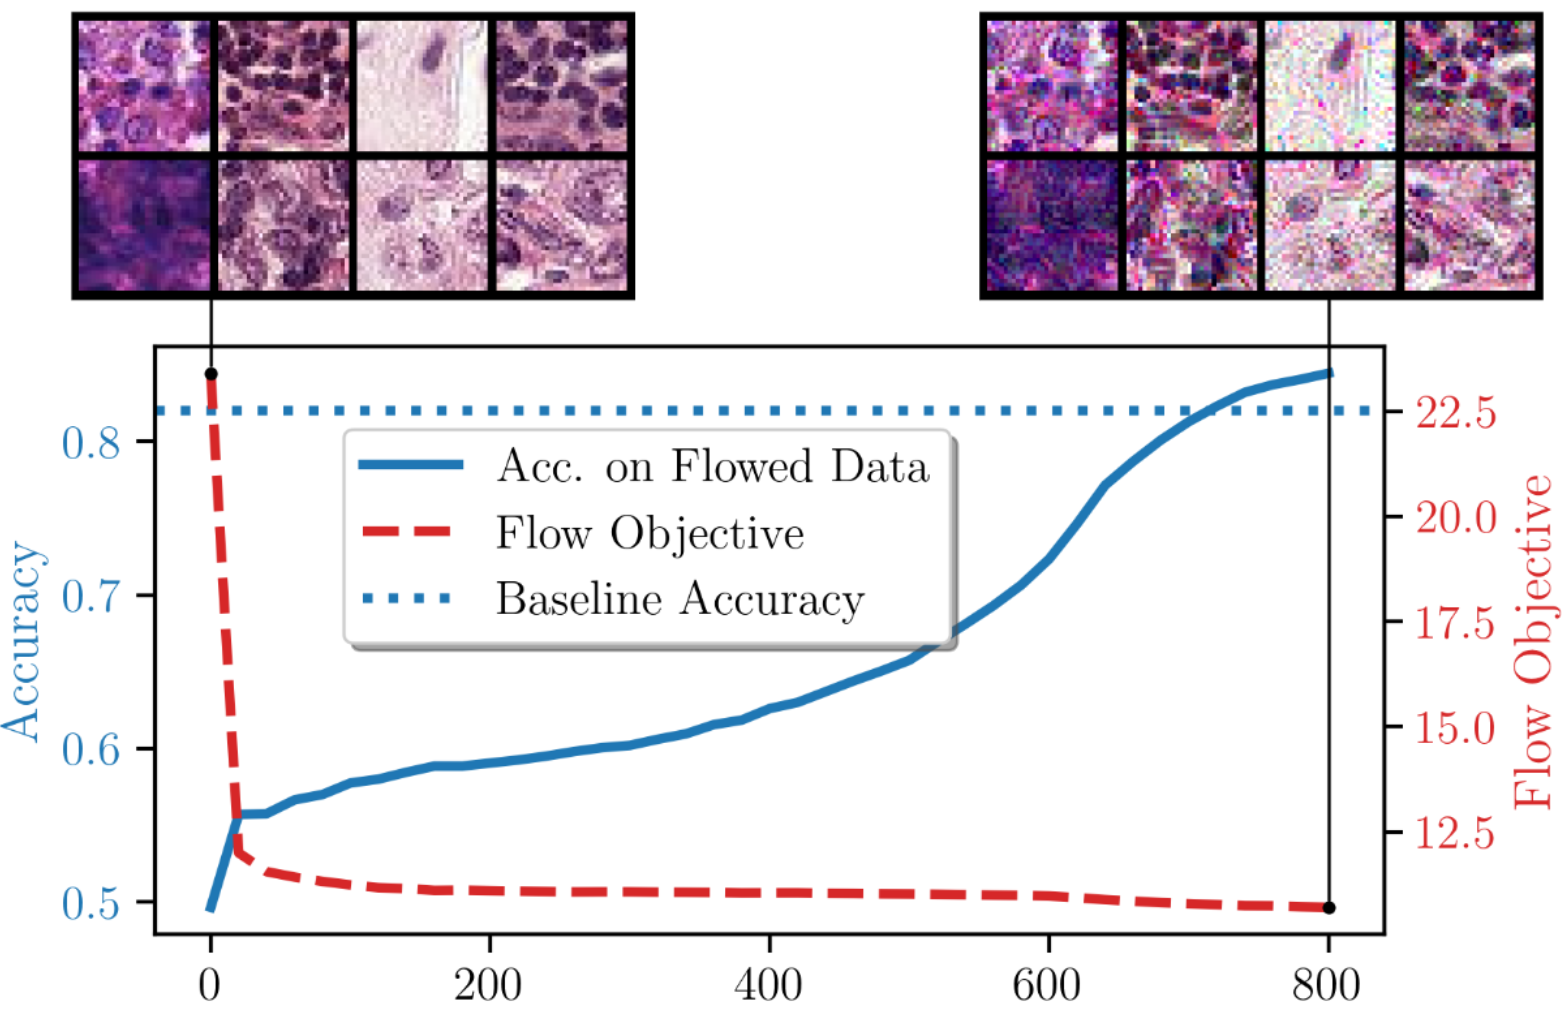
\includegraphics[width=0.7\linewidth]{chapters/petr_mokrov_s2/figs/model_repurposing.png}
\end{figure}


\section{Questions To Discussion}

\begin{itemize}
    \item Для решения каких задач можно использовать Dataset Dynamics (приведите примеры)?
    \item Какие геометрические свойства можно ввести в целевой (преобразованный) датасет с помощью потенциальной энергии $\olive{\cV(\rho)}$? с помощью энергии взаимодействия $\sunset{\cW(\rho)}$? (приведите примеры)
    \item Почему градиентный поток Вассерштайна $\partial_t \rho_t =  \divg{(\rho_t \nabla_{z} \fdv{F}{\rho}(\rho_t))}$ называется \textit{градиентным} потоком?
    \item В чём смысл первой вариации $\green{\fdv{F}{\rho}}(\rho)$?
\end{itemize}